\documentclass[tikz,border=10pt]{standalone}
\usetikzlibrary{calc,angles,quotes}

\begin{document}
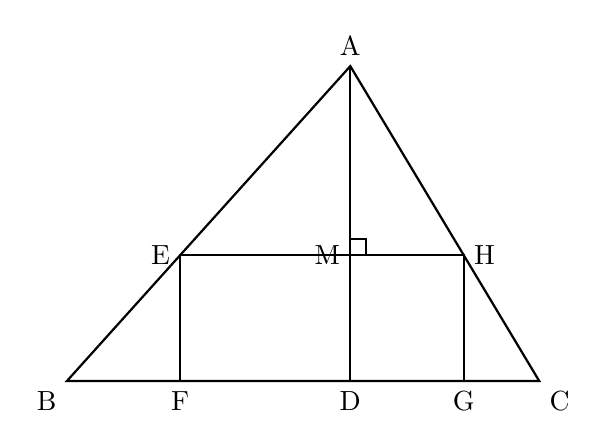
\begin{tikzpicture}[scale=2, thick]
    % 1. 定义顶点坐标
    \coordinate (B) at (0, 0);
    \coordinate (C) at (3, 0);
    \coordinate (A) at (1.8, 2);
    \coordinate (D) at (1.8, 0); % 高 AD 的底点

    % 2. 定义矩形顶点 (取 AD 上的 M 点高度为 0.8)
    \def\mheight{0.8}
    \coordinate (M) at (1.8, \mheight);
    
    % 计算 E 和 H 的位置 (利用相似三角形比例)
    % 线段 EH 在 AD 的垂直线上
    \coordinate (E) at ($(A)!{1-\mheight/2}!(B)$);
    \coordinate (H) at ($(A)!{1-\mheight/2}!(C)$);
    
    % F 和 G 是矩形在 BC 上的投影
    \coordinate (F) at (E |- B);
    \coordinate (G) at (H |- B);

    % 3. 绘制三角形轮廓
    \draw (A) -- (B) -- (C) -- cycle;
    
    % 4. 绘制高 AD 和辅助矩形
    \draw (A) -- (D);
    \draw (E) -- (H) -- (G) -- (F) -- cycle;

    % 5. 标记直角
    \draw ($(M)+(0.1,0)$) -- ($(M)+(0.1,0.1)$) -- ($(M)+(0,0.1)$);

    % 6. 标注点名
    \node[below left] at (B) {B};
    \node[below right] at (C) {C};
    \node[above] at (A) {A};
    \node[below] at (D) {D};
    \node[below] at (F) {F};
    \node[below] at (G) {G};
    \node[left] at (E) {E};
    \node[right] at (H) {H};
    \node[left] at (M) {M};

\end{tikzpicture}
\end{document}